\documentclass[preprint,12pt]{elsarticle}

\usepackage[T1]{fontenc}
\usepackage[utf8]{inputenc}
\usepackage{amsmath,amssymb}
\usepackage{booktabs}
\usepackage{graphicx}
\usepackage{tabularx}
\usepackage{array}
\usepackage{xcolor}
\usepackage{listings}
\usepackage{tikz}
\usetikzlibrary{arrows.meta,positioning}
\usepackage{lineno}
\usepackage{url}
\usepackage[hidelinks]{hyperref}

\journal{SoftwareX}

\definecolor{swxblue}{HTML}{245A8D}
\definecolor{swxlight}{HTML}{EAF2F8}
\definecolor{swxgray}{HTML}{4B5563}
\definecolor{swxred}{HTML}{B42318}
\newcommand{\swxreplace}[1]{\textcolor{swxred}{\textbf{[#1]}}}
\newcommand{\pkg}[1]{\texttt{#1}}
\newcommand{\code}[1]{\texttt{#1}}
\newcommand{\relLtwo}{\mathrm{rel}\,L_2}

% This file is intentionally the single human-editable metadata surface.
% Author and funding data were supplied by the corresponding author.
\newcommand{\AuthorOne}{Hyojin Park}
\newcommand{\AuthorTwo}{Nam-Hyun Yoo}
\newcommand{\AuthorThree}{Jinhong Yang}
\newcommand{\AffiliationOne}{Gyeongnam Intelligence Innovation Center (GIIC), Kyungnam University, 7 Gyeongnamdaehak-ro, Masanhappo-gu, Changwon 51767, Republic of Korea}
\newcommand{\AffiliationTwo}{Computer Engineering, Kyungnam University, Changwon 51767, Republic of Korea}
\newcommand{\AffiliationThree}{Department of Medical Information Technology, Inje University, Gimhae 50834, Republic of Korea}
\newcommand{\CorrespondingEmail}{jinhong@inje.ac.kr}
\newcommand{\CodeVersion}{v0.0.1}
\newcommand{\CodeURLText}{\url{https://github.com/Jinhong-Yang/CD-CureNO/tree/v0.0.1}}
\newcommand{\CodeLicenseText}{Apache License 2.0 (SPDX: Apache-2.0)}
\newcommand{\DocumentationURLText}{\url{https://github.com/Jinhong-Yang/CD-CureNO}}
\newcommand{\SupportEmailText}{jinhong@inje.ac.kr}
\newcommand{\FundingText}{This work was supported by the Institute of Information \& Communications Technology Planning \& Evaluation (IITP) -- Innovative Human Resource Development for Local Intellectualization program grant funded by the Korea government (MSIT) (IITP-2026-RS-2024-00436773).}
\newcommand{\CreditText}{\swxreplace{SOFTWAREX-REPLACE: CRediT author contribution statement}}
\newcommand{\AcknowledgementText}{None.}


\lstdefinestyle{softwarex}{
  basicstyle=\ttfamily\footnotesize,
  frame=single,
  rulecolor=\color{black!25},
  backgroundcolor=\color{black!2},
  breaklines=true,
  columns=fullflexible,
  keepspaces=true,
  showstringspaces=false,
  xleftmargin=0.4em,
  xrightmargin=0.4em
}
\lstset{style=softwarex}

\begin{document}

\begin{frontmatter}

\title{CD-CureNO: Reproducible software for restriction-preserving causal neural operators in composite curing}

\author[aff1]{\AuthorOne}
\author[aff2]{\AuthorTwo}
\author[aff3]{\AuthorThree\corref{cor1}}
\cortext[cor1]{Corresponding author}
\ead{\CorrespondingEmail}
\address[aff1]{\AffiliationOne}
\address[aff2]{\AffiliationTwo}
\address[aff3]{\AffiliationThree}

\begin{abstract}
CD-CureNO is a Python research-software stack for reproducible operator
learning in thermochemical composite curing. It audits legacy position-wise
ResFNO workflows, implements conservative one- and two-dimensional solvers,
creates immutable datasets and splits, trains joint and causal operators,
inflates one-dimensional checkpoints into restriction-preserving
two-dimensional models, and independently verifies saved experiments.
Scientific safeguards include train-only normalization, complete-case splits,
held-out firewalls, transactional run journals, hash-bound manifests, causal
future-perturbation tests, and conservative energy diagnostics. In staged
validation, a 512-case two-dimensional benchmark passed 27 solver checks and
deterministic replay, while checkpoint inflation preserved homogeneous
solutions to numerical tolerance. The package supports auditable development
without converting validation-only evidence into confirmatory claims.
\end{abstract}

\begin{keyword}
research software \sep neural operator \sep composite curing \sep
thermochemical simulation \sep reproducibility \sep causal machine learning
\end{keyword}

\end{frontmatter}

\linenumbers

\section*{Code metadata}

\begin{table}[!ht]
\centering
\small
\caption{SoftwareX code metadata. The C1--C8 labels and field meanings follow
the official SoftwareX original-software template, version 6 (March 2026).}
\label{tab:metadata}
\begin{tabularx}{\textwidth}{>{\raggedright\arraybackslash}p{0.07\textwidth}
                              >{\raggedright\arraybackslash}p{0.35\textwidth}
                              X}
\toprule
Nr & Code metadata description & Metadata \\
\midrule
C1 & Current code version & \CodeVersion \\
C2 & Permanent link to code/repository used for this code version & \CodeURLText \\
C3 & Legal code license & \CodeLicenseText \\
C4 & Code versioning system used & Git \\
C5 & Software code languages, tools, and services used & Python 3.10--3.12; PyTorch 2.13.0; NumPy 2.2.6; SciPy 1.15.3; pandas 2.3.3; PyArrow 25.0.0; Matplotlib 3.10.9; pytest 9.1.1 \\
C6 & Compilation requirements, operating environments, and dependencies &
Python package installed with \code{pip install -e ".[dev]"}; CPU execution is supported for audits and tests; CUDA is optional for model training; dependencies are pinned in \code{pyproject.toml}. \\
C7 & Link to developer documentation/manual & \DocumentationURLText \\
C8 & Support email for questions & \SupportEmailText \\
\bottomrule
\end{tabularx}
\end{table}

\section{Motivation and significance}

Thermochemical curing models connect an imposed air-temperature program to the
temperature and degree-of-cure fields inside a composite-tool assembly. These
fields matter because local thermal overshoot, cure gradients, and incomplete
cure can affect process design and final part quality. High-fidelity finite
element or finite-volume calculations are useful but costly when cure cycles,
heat-transfer coefficients, material parameters, and geometry must be varied.
Neural operators offer a function-to-function surrogate rather than a model
for one fixed input, and Fourier neural operators provide one influential
implementation of that idea~\cite{li2021fno}.

Existing composite-curing work already includes physics-informed neural
networks~\cite{niaki2021pinn}, residual neural operators~\cite{chen2023resfno},
and physics-informed neural operators~\cite{meng2023pino}. CD-CureNO therefore
does not claim novelty for using an FNO, jointly predicting temperature and
cure, or adding a physics loss. Its software problem is narrower and more
practical: how can a research team develop, transfer, evaluate, and report
cross-dimensional curing operators without losing the provenance and
scientific controls needed to interpret the result?

The motivating legacy ResFNO implementation learns one temporal operator at a
fixed through-thickness position and reconstructs a field by stacking up to 51
independently trained models~\cite{chen2021resfno,chen2023resfno}. A public
implementation is scientifically valuable, but direct reuse exposes common
research-code risks: normalization before splitting, inconsistent code paths,
batch-local metric aggregation, incomplete field outputs, and ambiguity about
whether a displayed position-by-time image is a jointly coupled spatial
operator. CD-CureNO provides a behaviorally faithful legacy path and a
separately named corrected path, then moves to a single joint 1+1-D model and a
true two-spatial-dimensional target. The terminology is enforced in code,
manifests, and reporting artifacts.

Lower-dimensional pretraining and boundary-to-domain lifting have become
important precedents for data-efficient operator learning
~\cite{hemmasian2024prelowd,kashi2024lpfno}. CD-CureNO adds software support
for a stronger engineering invariant: for laterally homogeneous coefficients,
initial conditions, and boundary data with zero lateral flux, the target model
should recover the source mapping when initialized. The implementation copies
the shared through-thickness and temporal computation, initializes new lateral
branches as zero residuals, and independently recreates every target tensor
before accepting an inflated checkpoint. A separate causal path uses dilated
temporal convolutions and a future-perturbation test, following the broader
principle that causal response models must exclude future inputs
~\cite{liu2024causal}.

The intended users are researchers in scientific machine learning, composite
manufacturing, and computational heat transfer who need more than model
classes. They need immutable split manifests, conservative reference solvers,
resumable runs, provenance-rich outputs, independent postflight checks, and a
claim boundary that distinguishes validation-only evidence from confirmatory
held-out results. CD-CureNO packages those concerns as one inspectable workflow.

\section{Software description}

\subsection{Software architecture}

CD-CureNO follows a staged artifact flow rather than a notebook-only workflow.
Figure~\ref{fig:architecture} summarizes the five principal layers. Data and
provenance enter through immutable manifests. Conservative solvers generate or
validate labels. Model modules implement joint, causal, and dimension-transfer
operators. Training modules provide resume support and single-writer
journals. Evaluation and reporting modules independently reconstruct metrics,
bind numbers to run identifiers, and fail closed when an integrity contract is
not satisfied.

\begin{figure}[!ht]
\centering
\resizebox{\textwidth}{!}{%
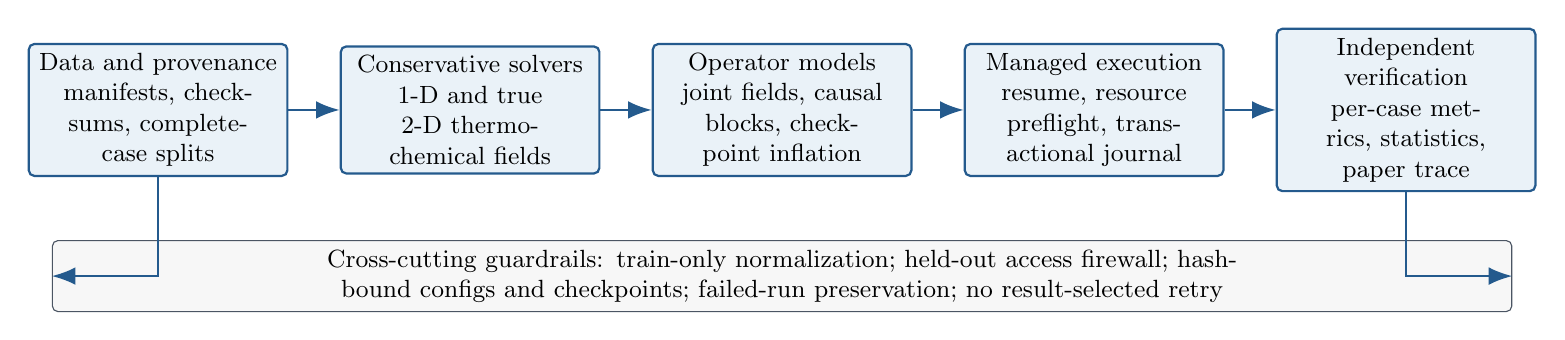
\begin{tikzpicture}[
  node distance=0.65cm,
  block/.style={draw=swxblue, rounded corners=2pt, thick, fill=swxlight,
                align=center, minimum height=1.35cm, text width=3.05cm,
                font=\small},
  audit/.style={draw=swxgray, rounded corners=2pt, fill=black!3,
                align=center, minimum height=0.72cm, text width=18.3cm,
                font=\small},
  arrow/.style={-{Latex[length=3mm]}, thick, draw=swxblue}
]
\node[block] (data) {Data and provenance\\manifests, checksums, complete-case splits};
\node[block, right=of data] (solver) {Conservative solvers\\1-D and true 2-D thermochemical fields};
\node[block, right=of solver] (model) {Operator models\\joint fields, causal blocks, checkpoint inflation};
\node[block, right=of model] (train) {Managed execution\\resume, resource preflight, transactional journal};
\node[block, right=of train] (report) {Independent verification\\per-case metrics, statistics, paper trace};
\draw[arrow] (data) -- (solver);
\draw[arrow] (solver) -- (model);
\draw[arrow] (model) -- (train);
\draw[arrow] (train) -- (report);
\node[audit, below=0.8cm of model] (guard) {Cross-cutting guardrails: train-only normalization; held-out access firewall; hash-bound configs and checkpoints; failed-run preservation; no result-selected retry};
\draw[arrow] (data.south) |- (guard.west);
\draw[arrow] (report.south) |- (guard.east);
\end{tikzpicture}%
}
\caption{CD-CureNO software architecture. Each stage emits inspectable
artifacts consumed by the next stage; cross-cutting guardrails are verified
again during independent aggregation and reporting.}
\label{fig:architecture}
\end{figure}

The package is organized under \pkg{src/cdcureno}. The \pkg{data} module
loads public and generated arrays, fits normalization on training cases only,
and exposes separate training shards and evaluation readers. The
\pkg{solvers} module implements conservative one- and two-dimensional
thermochemical integration with harmonic face conductance and Robin boundary
fluxes. The \pkg{models} module contains joint operators, causal temporal
blocks, target operators, ablations, and deterministic checkpoint-inflation
logic. The \pkg{training} module records configurations, environment and Git
state, histories, checkpoints, receipts, and process liveness. The
\pkg{evaluation} and \pkg{reporting} modules recompute complete-case metrics
from saved predictions and bind manuscript values to exact evidence.

\begin{table}[!ht]
\centering
\small
\caption{Major software functionality and its primary audit artifact.}
\label{tab:functionality}
\begin{tabularx}{\textwidth}{>{\raggedright\arraybackslash}p{0.19\textwidth}
                              >{\raggedright\arraybackslash}p{0.35\textwidth}
                              X}
\toprule
Function & User-facing capability & Audit output \\
\midrule
Legacy audit & Inspect upstream data shapes, splits, normalization, losses, and expected files without modifying the pinned source & JSON/Markdown inventory and regression tests \\
Reproducible training & Run exact, corrected, joint, and causal experiments with deterministic IDs and resume support & Resolved config, Git/environment snapshot, history, checkpoints, predictions, receipt \\
Conservative simulation & Generate one- and two-dimensional temperature/cure labels and validate energy closure, refinement, and extrusion & Per-case metadata, convergence tables, immutable manifests \\
Cross-dimensional transfer & Inflate a one-dimensional source into a target with copied shared tensors and zero-residual lateral adapters & Tensor mapping, tensor hashes, recreated target state, restriction metrics \\
Causality verification & Perturb all future input channels and compare every saved output on the unperturbed prefix & Cutoff-wise prefix differences and pass/fail contract \\
Independent reporting & Recompute per-case metrics, release frozen populations, run registered statistics, and trace manuscript values & Postflight reports, release receipts, statistics bundle, number-to-run trace \\
\bottomrule
\end{tabularx}
\end{table}

\subsection{Restriction-preserving and causal target construction}

The target model uses canonical input order
\([B,N_t,N_z,N_x,C_{\mathrm{in}}]\) and returns temperature and degree of
cure over the same time-space grid. For a laterally extruded source prediction,
the target is written conceptually as
\begin{equation}
  \widehat{T}_{2D}(x,z,t)
  = \operatorname{Lift}_{x}\!\left[\widehat{T}_{1D}(z,t)\right]
    + \Delta T_x(x,z,t).
\end{equation}
The new geometry projection and lateral adapter output factors are initialized
to zero. Consequently, homogeneous inputs recover the source computation at
initialization, up to floating-point ordering effects for \(N_x>1\). The
inflation report records copied tensors, initialized tensors, shape changes,
and hashes. A verifier then reconstructs the full untrained target from the
pinned source checkpoint, configuration, and seed; checking model outputs
alone is insufficient because a trained target could accidentally appear
lateral-invariant on a small test.

The structurally causal target contains eight dilated temporal convolutions
and no temporal FFT modules. Causality is checked by perturbing every input
channel after several cutoffs and requiring all temperature, residual,
degree-of-cure, and cure-rate prefixes to remain unchanged. Cure is represented
through a nonnegative latent rate integrated into a bounded monotone state,
while conservative residuals use finite-volume-compatible fluxes rather than
global derivatives across a material interface.

\subsection{Scientific and execution safeguards}

Every expensive run has a resolved configuration, data checksums, random seed,
environment snapshot, checkpoint history, per-case metrics, and physical-unit
predictions. Splits are defined by complete cure cycle or complete simulation
case; spatial and temporal grid points are never treated as independent
samples. The package preserves failed and superseded runs, and result indices
record only independently verified completions. Managed execution uses a
single-writer lease and journal so interruption cannot silently change the
selected checkpoint population.

The reporting layer separates structural, validation-only, descriptive, and
confirmatory evidence. The current SoftwareX article uses only passed P0--P5
software-validation artifacts. It does not use the unfinished P6 held-out
campaign to claim superiority, label savings, state of the art, or broad
source-seed invariance.

\section{Illustrative examples}

\subsection{Installation and audit}

The repository targets Python 3.10--3.12. A clean editable installation and
CPU test run are:

\begin{lstlisting}[language=bash]
python -m venv .venv
.venv/Scripts/python -m pip install -e ".[dev]"
.venv/Scripts/python -m pytest -q
\end{lstlisting}

The legacy audit is read-only and supports a dry run:

\begin{lstlisting}[language=bash]
.venv/Scripts/python scripts/audit_legacy_repo.py \
  --repo-root external/ResFNO \
  --output-dir outputs/audit \
  --dry-run
\end{lstlisting}

The implemented CLI also exposes auditable exact, corrected, joint
factorized, and joint causal training modes. Independent evaluation reloads a
saved run by identifier and recomputes its complete-case metrics.

\subsection{Conservative two-dimensional benchmark}

The two-dimensional workflow separates plan generation from label generation,
which allows users to review case families and split semantics before solving:

\begin{lstlisting}[language=bash]
.venv/Scripts/python scripts/generate_p4_2d.py \
  --tier core --plan-only
.venv/Scripts/python scripts/validate_p4_solver.py
.venv/Scripts/python scripts/verify_p4_gate.py
\end{lstlisting}

The frozen core benchmark contains 512 cases with temperature/cure field shape
\([512,112,50,40]\). The production solver passed 27 pre-specified checks;
all cases completed, the maximum relative global energy residual was
\(1.345\times10^{-12}\), and 11 cases selected from plan metadata reproduced
their saved float32 slice hashes exactly. The independent SciPy-BDF check
reassembled fluxes and time integration but shared the grid, material values,
and cure law, so it is not described as a fully independent external solver.

\subsection{Checkpoint inflation and restriction verification}

The causal inflation path can execute all checks in memory before writing:

\begin{lstlisting}[language=bash]
.venv/Scripts/python \
  scripts/inflate_causal_1d_to_2d_checkpoint.py --dry-run
.venv/Scripts/python \
  scripts/verify_p5_causal_restriction.py --dry-run
\end{lstlisting}

For the saved causal target, 100 source tensors were copied bitwise and 17
target tensors were initialized; the complete 117-tensor state matched a
deterministic reconstruction. On the actual homogeneous P4 validation input,
temperature restriction relative \(L_2\) and lateral-invariance scores were
\(3.33\times10^{-8}\) and \(1.76\times10^{-8}\), respectively. The maximum
future-prefix difference was exactly zero across three cutoffs, four output
fields, and perturbations to all 20 target channels. These checks use
label-free homogeneous inputs and establish initialization behavior and
architectural causality, not predictive superiority.

\subsection{Joint-field reconstruction}

Figure~\ref{fig:p2temperature} illustrates an output of the earlier joint
1+1-D stage. The case identifier was fixed before plotting, and shared color
scales permit visual comparison. The figure is deliberately labelled as a
through-thickness-by-time result, not a true two-spatial-dimensional field.

\begin{figure}[!ht]
\centering
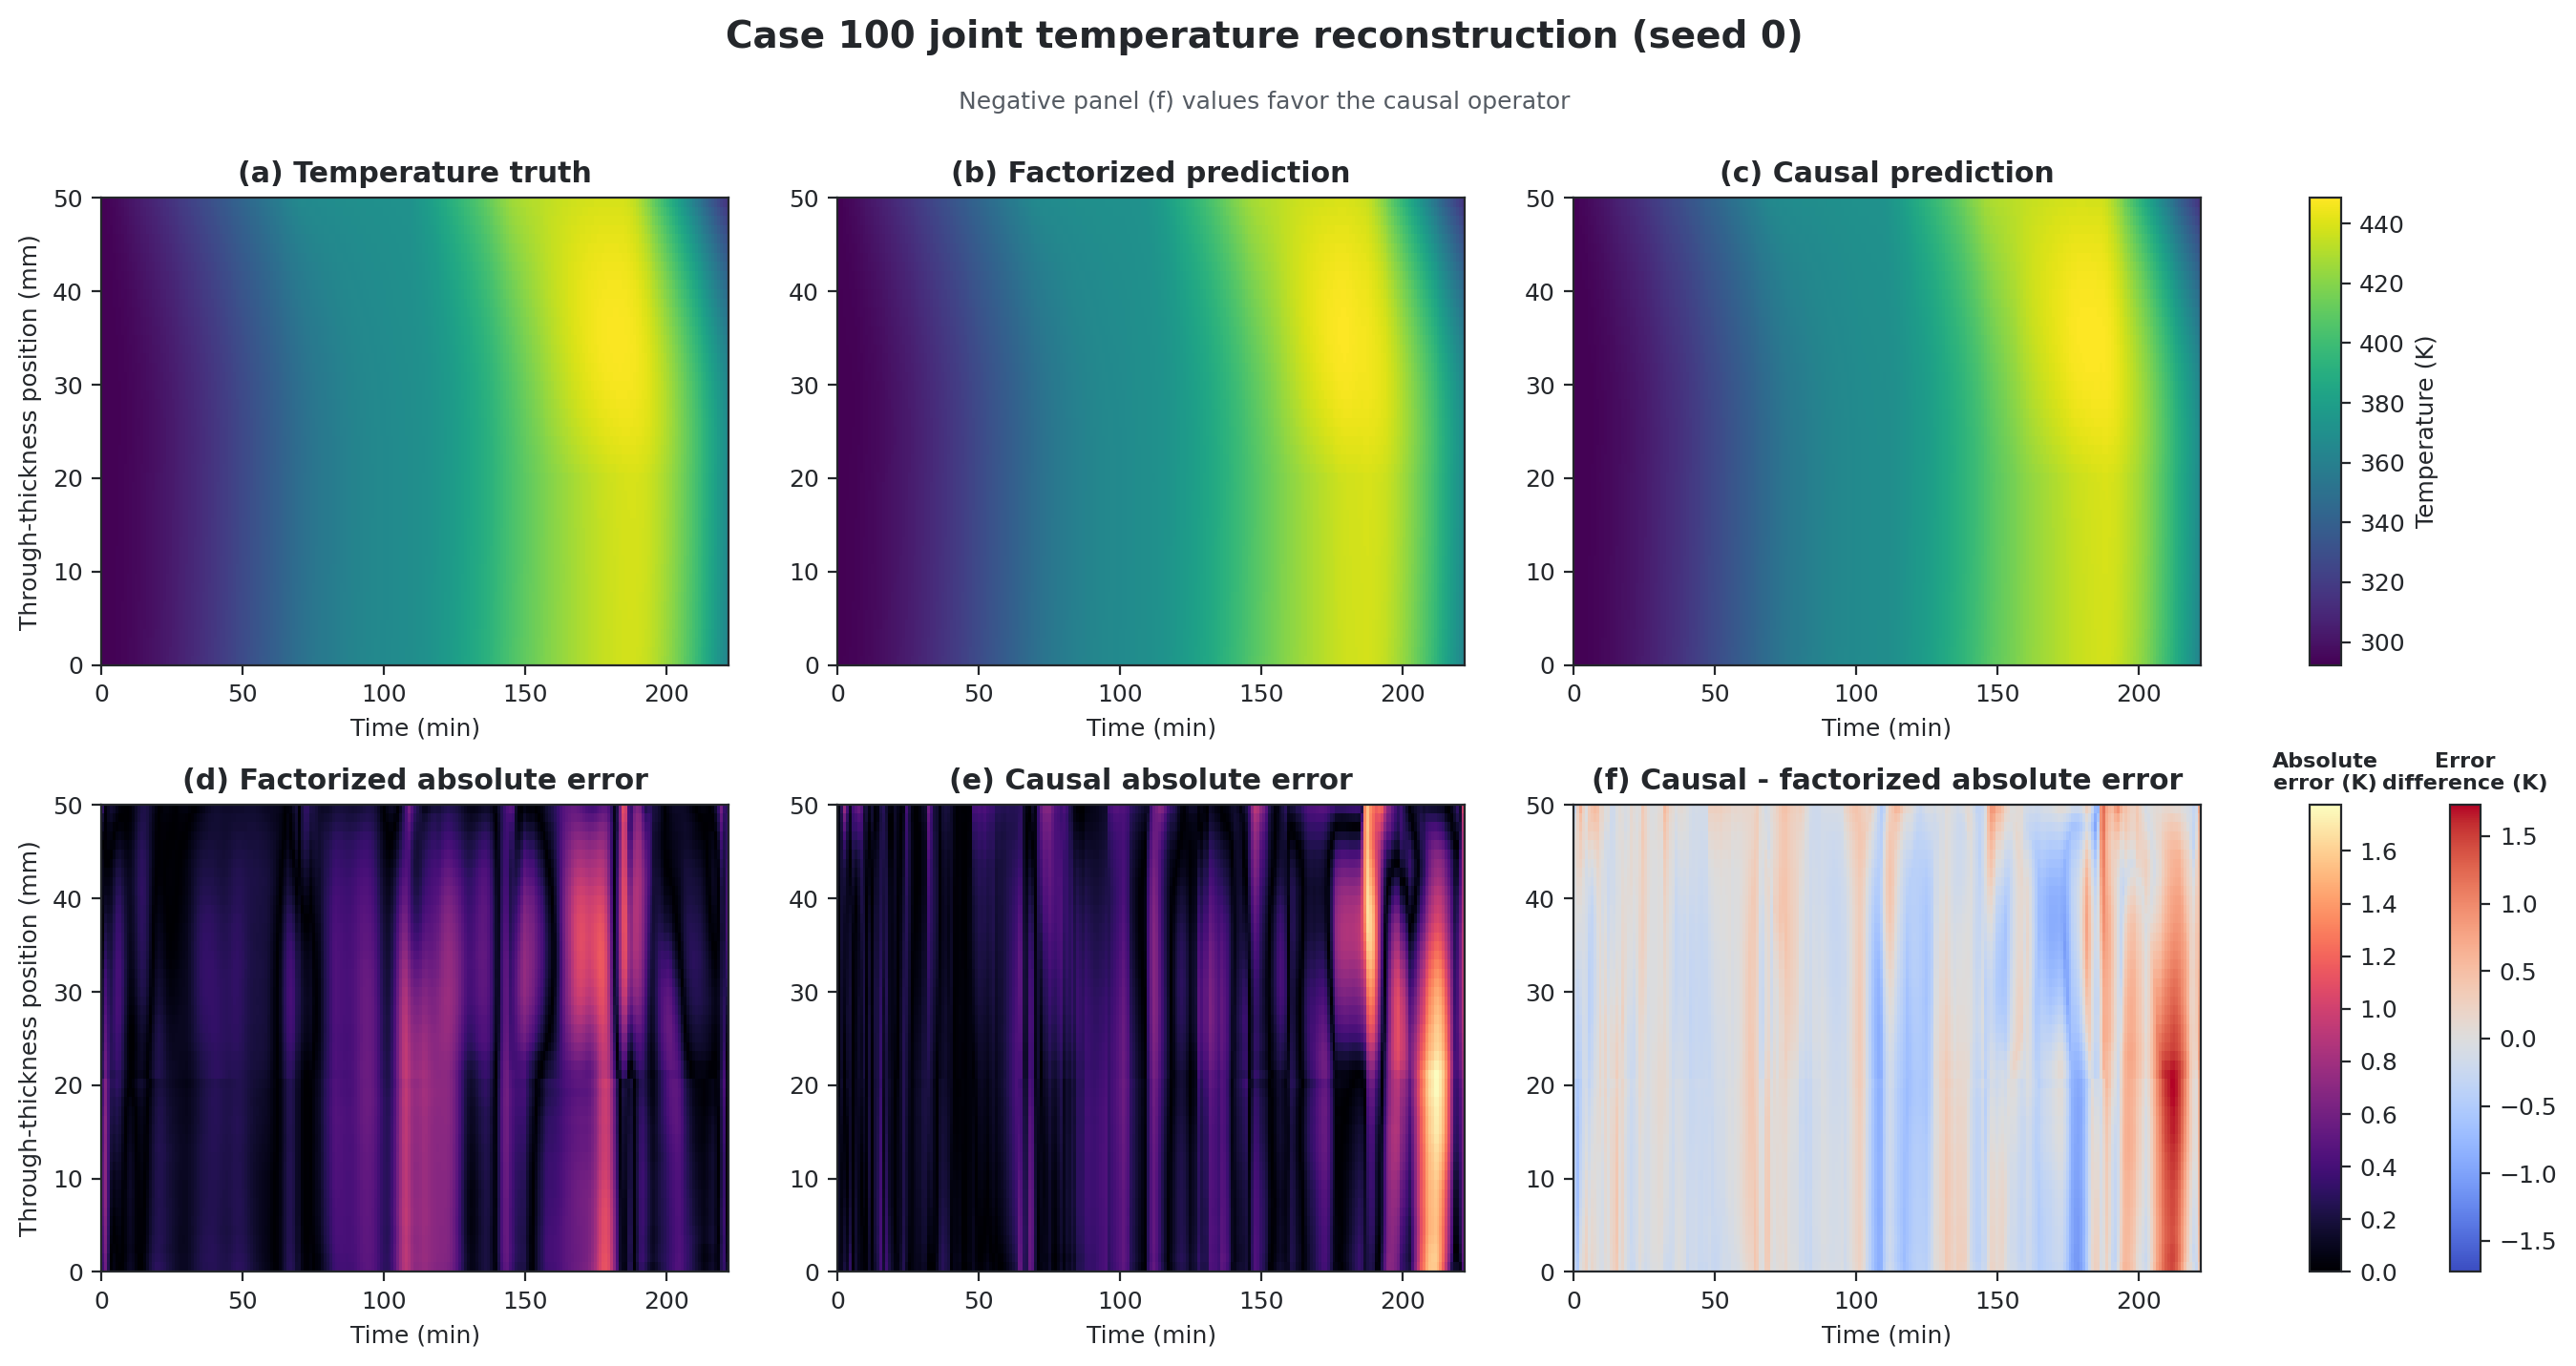
\includegraphics[width=\textwidth]{figures/p2_case100_temperature.png}
\caption{Representative joint 1+1-D temperature reconstruction for fixed test
case 100 and seed 0. The factorized and causal models were selected by the
validation objective. This single-case display is descriptive and does not
establish statistical superiority.}
\label{fig:p2temperature}
\end{figure}

The factorized and causal joint models used 198,282 and 225,162 parameters,
respectively, compared with 15,076,467 parameters across 51 independently
trained legacy models. Their seed-0 complete-case temperature relative
\(L_2\) means were 0.001192 and 0.001310; all saved cure predictions respected
bounds and monotonicity, and the causal model showed exactly zero prefix
change in its fixed future-perturbation test. These are staged, one-seed
validation results and are included only to demonstrate the software's
joint-field and causality workflows.

\begin{table}[!ht]
\centering
\small
\caption{Evidence used to validate the current software release. Performance
entries marked descriptive or validation-only are not confirmatory claims.}
\label{tab:validation}
\begin{tabularx}{\textwidth}{>{\raggedright\arraybackslash}p{0.11\textwidth}
                              >{\raggedright\arraybackslash}p{0.25\textwidth}
                              >{\raggedright\arraybackslash}p{0.30\textwidth}
                              X}
\toprule
Stage & Population & Verified result & Claim boundary \\
\midrule
P0--P1 & Public Case1; 200 cycles, 51 positions, 223 times & Nine legacy defects regression-tested; exact and corrected field workflows independently reconstructed & Reproduction and audit behavior; no corrected-accuracy gain claimed \\
P2 & 125 complete test cases; seed 0 & Joint factorized \(\relLtwo=0.001192\); causal \(\relLtwo=0.001310\); zero causal prefix change & Descriptive one-seed phase gate; 1+1-D only \\
P3 & 200 public solver cases & Mean temperature \(\relLtwo=0.001143\); maximum global energy residual \(5.304\times10^{-13}\) & Open-solver agreement; proprietary COMSOL parity not established \\
P4 & 512 generated true-2-D cases & 27 solver checks passed; zero failed cases; deterministic replay passed & Public-data-anchored numerical benchmark; no geometry-OOD claim \\
P5 & Label-free restriction tests and one-seed validation pilot & Causal restriction and future-invariance gates passed; transfer pilot passed at budgets 8 and 16 & Initialization and functionality evidence; pilot comparison is validation-only \\
\bottomrule
\end{tabularx}
\end{table}

\section{Impact}

CD-CureNO's primary present impact is methodological infrastructure. First, it
makes the behavior of a legacy curing-operator codebase inspectable. Exact and
corrected paths remain separately named, allowing a researcher to reproduce
reported behavior without quietly repairing it, then compare against a fairer
implementation. The audit detected and regression-tested nine issues,
including normalization leakage, an unused smoothness term, inconsistent
function calls, and incomplete field output expectations. This reduces the
risk that later scientific conclusions rest on undocumented implementation
differences.

Second, the software connects conservative simulation to operator learning in
one repository. The one-dimensional solver is checked against 200 public
cases, refinement, and energy closure. The two-dimensional solver is checked
against an extruded one-dimensional limit, a method-of-lines BDF calculation,
energy invariants, deterministic replay, and complete dataset manifests. The
same case identifiers, masks, coordinates, and hashes then flow into training
and evaluation. This shared contract is useful for studying transfer without
treating generated labels as unquestioned ground truth.

Third, CD-CureNO turns restriction preservation and causal response into
executable tests. A researcher can inspect which tensors were copied, which
were initialized, whether a lateral zero mode can change the source mapping,
and whether any future input changes a predicted prefix. These facilities can
support new questions about when lower-dimensional pretraining helps, when the
benefit disappears as target labels increase, and whether physical invariants
improve worst-case behavior. They can also be reused as test patterns for
other evolution equations with a known dimensional-reduction limit.

Fourth, the managed-run and reporting layers preserve negative evidence.
Interrupted sessions, failed development variants, superseded cohorts, and
unknown wall-time intervals are retained rather than zero-imputed or replaced.
Manuscript tokens can be resolved only from a verified statistics pointer and
an explicit run population. This supports the software-citation principle
that a cited version should be identifiable and recoverable
~\cite{smith2016software}.

The current repository has no defensible public download, user, or commercial
adoption count, so this article makes no adoption claim. At submission, the
tagged GitHub release, license, README, and developer documentation named in
Table~\ref{tab:metadata} must be public. CD-CureNO is released under the
OSI-approved Apache License 2.0, which permits use, modification, and
redistribution, including commercial use, subject to its terms. External/ResFNO
code and data must not be redistributed under an assumed license; the release
should retain only the submodule pointer or documented acquisition/checksum
workflow allowed by the upstream terms.

Scientific scope also remains bounded. The canonical benchmark uses a
rectangular grid, reference-temperature conductivity, and a unidirectional
material model. Geometry OOD is deferred. The BDF cross-check is independent
in flux assembly and integration but shares physical inputs. P2 and P5 model
comparisons are one-seed or validation-only. The unfinished P6 confirmatory
campaign and context-only external sources are not used in this paper as
evidence of superiority, broad generalization, or experimental validation.

\section{Conclusions}

CD-CureNO packages the complete research workflow needed to study
cross-dimensional neural operators for composite curing: legacy audit,
conservative one- and two-dimensional solvers, immutable data manifests,
joint and causal models, deterministic restriction-preserving inflation,
resumable managed execution, independent evaluation, and traceable reporting.
The current validation demonstrates software correctness and staged scientific
readiness while explicitly preserving the boundary between validation and
confirmation. The package is intended to make future claims easier to audit,
reproduce, narrow, or reject when the evidence requires it.

\section*{Data and code availability}

The exact software version described in this article is available from the
following repository:

\CodeURLText

The open-source release license is:

\CodeLicenseText

Generated arrays, public-data acquisition steps, manifests, and redistribution
restrictions are documented in the release README. Upstream ResFNO artifacts
remain subject to their own license status and are not relicensed by CD-CureNO.

\section*{CRediT author statement}
\CreditText

\section*{Funding}
\FundingText

\section*{Acknowledgements}
\AcknowledgementText

\section*{Declaration of competing interest}
The authors declare that they have no known competing financial interests or
personal relationships that could have appeared to influence the work reported
in this paper. % SOFTWAREX-REPLACE: authors must confirm this statement.

\bibliographystyle{elsarticle-num}
\bibliography{references}

\end{document}
